\begin{figure}[htb!]
  \centering
  \begin{subfigure}[b]{0.38\textwidth}
    \centering
    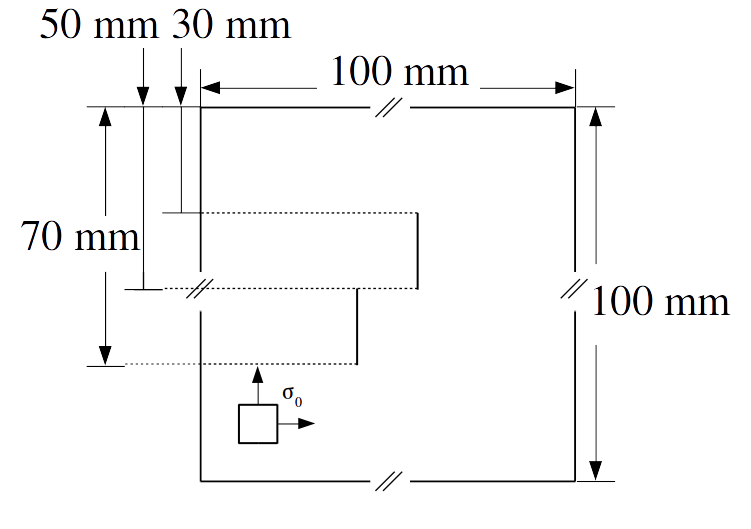
\includegraphics[width=\textwidth,scale=0.5]{Chapter4/figures/biaxial_dimensions.png}
    \caption{}
    \label{fig: Chapter4/biaxial_dimensions}
  \end{subfigure}
  \begin{subfigure}[b]{0.325\textwidth}
    \centering
    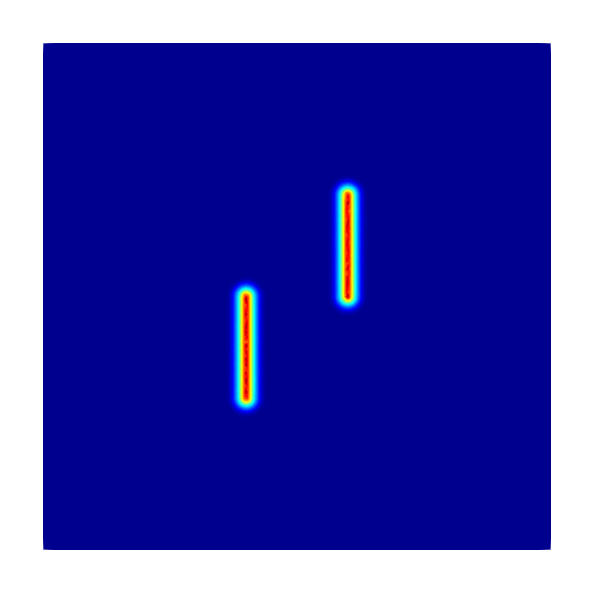
\includegraphics[width=0.73\textwidth,scale=0.5]{Chapter4/figures/biaxial_initial.png}
    \caption{}
    \label{fig: Chapter4/biaxial_initial}
  \end{subfigure}
  \begin{subfigure}[b]{0.07\textwidth}
    \centering
    \caption*{d}
    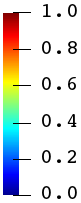
\includegraphics[width=\textwidth]{Chapter4/figures/jet_vertical.png}
    \vspace{0.15in}
  \end{subfigure}
  \caption[Dimensions and boundary conditions of a thin plate with two parallel initial cracks.]{(a) Dimensions and boundary conditions of a thin plate with two parallel initial cracks. (b) The initial cracks are represented by an initial phase field.}
  \label{fig: Chapter4/biaxial_schematic}
\end{figure}
